\documentclass[twoside]{book}

% Packages required by doxygen
\usepackage{fixltx2e}
\usepackage{calc}
\usepackage{doxygen}
\usepackage[export]{adjustbox} % also loads graphicx
\usepackage{graphicx}
\usepackage[utf8]{inputenc}
\usepackage{makeidx}
\usepackage{multicol}
\usepackage{multirow}
\PassOptionsToPackage{warn}{textcomp}
\usepackage{textcomp}
\usepackage[nointegrals]{wasysym}
\usepackage[table]{xcolor}

% Font selection
\usepackage[T1]{fontenc}
\usepackage[scaled=.90]{helvet}
\usepackage{courier}
\usepackage{amssymb}
\usepackage{sectsty}
\renewcommand{\familydefault}{\sfdefault}
\allsectionsfont{%
  \fontseries{bc}\selectfont%
  \color{darkgray}%
}
\renewcommand{\DoxyLabelFont}{%
  \fontseries{bc}\selectfont%
  \color{darkgray}%
}
\newcommand{\+}{\discretionary{\mbox{\scriptsize$\hookleftarrow$}}{}{}}

% Page & text layout
\usepackage{geometry}
\geometry{%
  a4paper,%
  top=2.5cm,%
  bottom=2.5cm,%
  left=2.5cm,%
  right=2.5cm%
}
\tolerance=750
\hfuzz=15pt
\hbadness=750
\setlength{\emergencystretch}{15pt}
\setlength{\parindent}{0cm}
\setlength{\parskip}{3ex plus 2ex minus 2ex}
\makeatletter
\renewcommand{\paragraph}{%
  \@startsection{paragraph}{4}{0ex}{-1.0ex}{1.0ex}{%
    \normalfont\normalsize\bfseries\SS@parafont%
  }%
}
\renewcommand{\subparagraph}{%
  \@startsection{subparagraph}{5}{0ex}{-1.0ex}{1.0ex}{%
    \normalfont\normalsize\bfseries\SS@subparafont%
  }%
}
\makeatother

% Headers & footers
\usepackage{fancyhdr}
\pagestyle{fancyplain}
\fancyhead[LE]{\fancyplain{}{\bfseries\thepage}}
\fancyhead[CE]{\fancyplain{}{}}
\fancyhead[RE]{\fancyplain{}{\bfseries\leftmark}}
\fancyhead[LO]{\fancyplain{}{\bfseries\rightmark}}
\fancyhead[CO]{\fancyplain{}{}}
\fancyhead[RO]{\fancyplain{}{\bfseries\thepage}}
\fancyfoot[LE]{\fancyplain{}{}}
\fancyfoot[CE]{\fancyplain{}{}}
\fancyfoot[RE]{\fancyplain{}{\bfseries\scriptsize Generated by Doxygen }}
\fancyfoot[LO]{\fancyplain{}{\bfseries\scriptsize Generated by Doxygen }}
\fancyfoot[CO]{\fancyplain{}{}}
\fancyfoot[RO]{\fancyplain{}{}}
\renewcommand{\footrulewidth}{0.4pt}
\renewcommand{\chaptermark}[1]{%
  \markboth{#1}{}%
}
\renewcommand{\sectionmark}[1]{%
  \markright{\thesection\ #1}%
}

% Indices & bibliography
\usepackage{natbib}
\usepackage[titles]{tocloft}
\setcounter{tocdepth}{3}
\setcounter{secnumdepth}{5}
\makeindex

% Hyperlinks (required, but should be loaded last)
\usepackage{ifpdf}
\ifpdf
  \usepackage[pdftex,pagebackref=true]{hyperref}
\else
  \usepackage[ps2pdf,pagebackref=true]{hyperref}
\fi
\hypersetup{%
  colorlinks=true,%
  linkcolor=blue,%
  citecolor=blue,%
  unicode%
}

% Custom commands
\newcommand{\clearemptydoublepage}{%
  \newpage{\pagestyle{empty}\cleardoublepage}%
}

\usepackage{caption}
\captionsetup{labelsep=space,justification=centering,font={bf},singlelinecheck=off,skip=4pt,position=top}

%===== C O N T E N T S =====

\begin{document}

% Titlepage & ToC
\hypersetup{pageanchor=false,
             bookmarksnumbered=true,
             pdfencoding=unicode
            }
\pagenumbering{roman}
\begin{titlepage}
\vspace*{7cm}
\begin{center}%
{\Large max7219 \\[1ex]\large 0.\+9 (last modified 20-\/06-\/2016) }\\
\vspace*{1cm}
{\large Generated by Doxygen 1.8.11}\\
\end{center}
\end{titlepage}
\clearemptydoublepage
\tableofcontents
\clearemptydoublepage
\pagenumbering{arabic}
\hypersetup{pageanchor=true}

%--- Begin generated contents ---
\chapter{max7219\+L\+ED}
\label{md_README}
\hypertarget{md_README}{}
Library for the max7219 chip for use with L\+ED matrices on the Arduino Due. This library is meant to be used with hwlib and bmptk. 
\chapter{Hierarchical Index}
\section{Class Hierarchy}
This inheritance list is sorted roughly, but not completely, alphabetically\+:\begin{DoxyCompactList}
\item \contentsline{section}{monochrome\+Display}{\pageref{classmonochrome_display}}{}
\begin{DoxyCompactList}
\item \contentsline{section}{max7219\+L\+ED}{\pageref{classmax7219_l_e_d}}{}
\end{DoxyCompactList}
\end{DoxyCompactList}

\chapter{Class Index}
\section{Class List}
Here are the classes, structs, unions and interfaces with brief descriptions\+:\begin{DoxyCompactList}
\item\contentsline{section}{\hyperlink{classmax7219_l_e_d}{max7219\+L\+ED} \\*Max7219\+L\+ED class }{\pageref{classmax7219_l_e_d}}{}
\item\contentsline{section}{\hyperlink{classmonochrome_display}{monochrome\+Display} }{\pageref{classmonochrome_display}}{}
\end{DoxyCompactList}

\chapter{File Index}
\section{File List}
Here is a list of all documented files with brief descriptions\+:\begin{DoxyCompactList}
\item\contentsline{section}{\hyperlink{max7219_l_e_d_8cpp}{max7219\+L\+E\+D.\+cpp} }{\pageref{max7219_l_e_d_8cpp}}{}
\item\contentsline{section}{\hyperlink{max7219_l_e_d_8hpp}{max7219\+L\+E\+D.\+hpp} }{\pageref{max7219_l_e_d_8hpp}}{}
\item\contentsline{section}{\hyperlink{max7219_l_e_dconstants_8hpp}{max7219\+L\+E\+Dconstants.\+hpp} }{\pageref{max7219_l_e_dconstants_8hpp}}{}
\item\contentsline{section}{\hyperlink{monochrome_8hpp}{monochrome.\+hpp} }{\pageref{monochrome_8hpp}}{}
\end{DoxyCompactList}

\chapter{Class Documentation}
\hypertarget{classmax7219_l_e_d}{}\section{max7219\+L\+ED Class Reference}
\label{classmax7219_l_e_d}\index{max7219\+L\+ED@{max7219\+L\+ED}}


\hyperlink{classmax7219_l_e_d}{max7219\+L\+ED} class  




{\ttfamily \#include $<$max7219\+L\+E\+D.\+hpp$>$}

Inheritance diagram for max7219\+L\+ED\+:\begin{figure}[H]
\begin{center}
\leavevmode
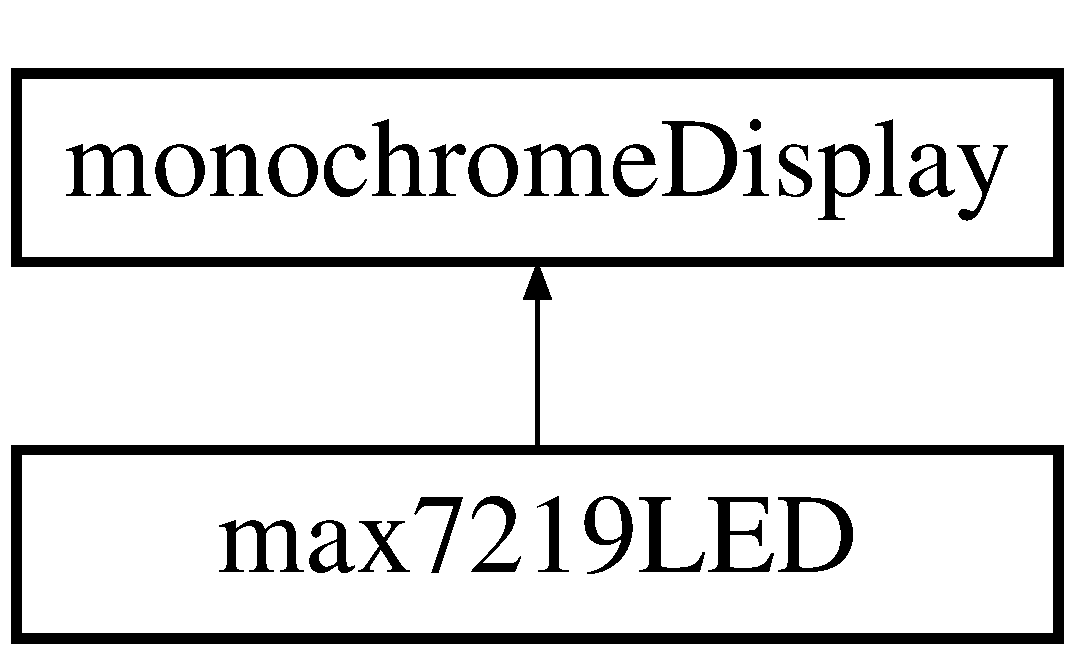
\includegraphics[height=2.000000cm]{classmax7219_l_e_d}
\end{center}
\end{figure}
\subsection*{Public Member Functions}
\begin{DoxyCompactItemize}
\item 
\hyperlink{classmax7219_l_e_d_a3f13dbd1dd54e3d3ce0148c1119273e5}{max7219\+L\+ED} (hwlib\+::target\+::pin\+\_\+out clk, hwlib\+::target\+::pin\+\_\+out din, hwlib\+::target\+::pin\+\_\+out cs, const int \&size\+\_\+x=\hyperlink{max7219_l_e_dconstants_8hpp_a2a4cf20d00f170bb1778318f645ab6cb}{L\+E\+D\+M\+A\+T\+R\+I\+X\+\_\+\+S\+I\+ZE}, const int \&size\+\_\+y=\hyperlink{max7219_l_e_dconstants_8hpp_a2a4cf20d00f170bb1778318f645ab6cb}{L\+E\+D\+M\+A\+T\+R\+I\+X\+\_\+\+S\+I\+ZE})
\item 
void \hyperlink{classmax7219_l_e_d_a6ce14869c58cf742e39e16620a4a724f}{draw\+Pixel} (int x, int y, int matrix\mbox{[}\hyperlink{max7219_l_e_dconstants_8hpp_a2a4cf20d00f170bb1778318f645ab6cb}{L\+E\+D\+M\+A\+T\+R\+I\+X\+\_\+\+S\+I\+ZE}+1\mbox{]}\mbox{[}(\hyperlink{max7219_l_e_dconstants_8hpp_a2a4cf20d00f170bb1778318f645ab6cb}{L\+E\+D\+M\+A\+T\+R\+I\+X\+\_\+\+S\+I\+ZE} $\ast$\hyperlink{max7219_l_e_dconstants_8hpp_aa3f1c3f51823e34beb0682e7f799793b}{L\+E\+D\+M\+A\+T\+R\+I\+X\+\_\+\+A\+M\+O\+U\+NT})+1\mbox{]}, int data=1) override
\begin{DoxyCompactList}\small\item\em Sets and draws a single pixel. \end{DoxyCompactList}\item 
void \hyperlink{classmax7219_l_e_d_a5ea755271f6306d1f0e97ec1f7c2c7c0}{clear} (int matrix\mbox{[}\hyperlink{max7219_l_e_dconstants_8hpp_a2a4cf20d00f170bb1778318f645ab6cb}{L\+E\+D\+M\+A\+T\+R\+I\+X\+\_\+\+S\+I\+ZE}+1\mbox{]}\mbox{[}(\hyperlink{max7219_l_e_dconstants_8hpp_a2a4cf20d00f170bb1778318f645ab6cb}{L\+E\+D\+M\+A\+T\+R\+I\+X\+\_\+\+S\+I\+ZE} $\ast$\hyperlink{max7219_l_e_dconstants_8hpp_aa3f1c3f51823e34beb0682e7f799793b}{L\+E\+D\+M\+A\+T\+R\+I\+X\+\_\+\+A\+M\+O\+U\+NT})+1\mbox{]}) override
\begin{DoxyCompactList}\small\item\em Clears the matrix and screen. \end{DoxyCompactList}\item 
void \hyperlink{classmax7219_l_e_d_abb0f536db36aa950bc189416d65db6a7}{initialise} (int matrix\mbox{[}\hyperlink{max7219_l_e_dconstants_8hpp_a2a4cf20d00f170bb1778318f645ab6cb}{L\+E\+D\+M\+A\+T\+R\+I\+X\+\_\+\+S\+I\+ZE}+1\mbox{]}\mbox{[}(\hyperlink{max7219_l_e_dconstants_8hpp_a2a4cf20d00f170bb1778318f645ab6cb}{L\+E\+D\+M\+A\+T\+R\+I\+X\+\_\+\+S\+I\+ZE} $\ast$\hyperlink{max7219_l_e_dconstants_8hpp_aa3f1c3f51823e34beb0682e7f799793b}{L\+E\+D\+M\+A\+T\+R\+I\+X\+\_\+\+A\+M\+O\+U\+NT})+1\mbox{]})
\begin{DoxyCompactList}\small\item\em initialise max7219 chip \end{DoxyCompactList}\item 
void \hyperlink{classmax7219_l_e_d_af913d07107bfc902dc66af95ead59f21}{send\+\_\+repeated\+\_\+data} (const uint16\+\_\+t data, const uint8\+\_\+t repeat)
\begin{DoxyCompactList}\small\item\em Send repeated data. \end{DoxyCompactList}\item 
void \hyperlink{classmax7219_l_e_d_ae15df95125db9c4efb33f19720c893a0}{shift\+\_\+repeated\+\_\+data} (const uint16\+\_\+t data, const uint8\+\_\+t repeat)
\begin{DoxyCompactList}\small\item\em Shift repeated data. \end{DoxyCompactList}\item 
void \hyperlink{classmax7219_l_e_d_a651b73c3236443e478785f4a3e180b3a}{set\+Pixel} (int x, int y, int matrix\mbox{[}\hyperlink{max7219_l_e_dconstants_8hpp_a2a4cf20d00f170bb1778318f645ab6cb}{L\+E\+D\+M\+A\+T\+R\+I\+X\+\_\+\+S\+I\+ZE}+1\mbox{]}\mbox{[}(\hyperlink{max7219_l_e_dconstants_8hpp_a2a4cf20d00f170bb1778318f645ab6cb}{L\+E\+D\+M\+A\+T\+R\+I\+X\+\_\+\+S\+I\+ZE} $\ast$\hyperlink{max7219_l_e_dconstants_8hpp_aa3f1c3f51823e34beb0682e7f799793b}{L\+E\+D\+M\+A\+T\+R\+I\+X\+\_\+\+A\+M\+O\+U\+NT})+1\mbox{]}, int data=1)
\begin{DoxyCompactList}\small\item\em Sets a pixel in the matrix. \end{DoxyCompactList}\item 
void \hyperlink{classmax7219_l_e_d_ace27bb3d99143c9c70cfead632e93f89}{draw\+Screen} (int matrix\mbox{[}\hyperlink{max7219_l_e_dconstants_8hpp_a2a4cf20d00f170bb1778318f645ab6cb}{L\+E\+D\+M\+A\+T\+R\+I\+X\+\_\+\+S\+I\+ZE}+1\mbox{]}\mbox{[}(\hyperlink{max7219_l_e_dconstants_8hpp_a2a4cf20d00f170bb1778318f645ab6cb}{L\+E\+D\+M\+A\+T\+R\+I\+X\+\_\+\+S\+I\+ZE} $\ast$\hyperlink{max7219_l_e_dconstants_8hpp_aa3f1c3f51823e34beb0682e7f799793b}{L\+E\+D\+M\+A\+T\+R\+I\+X\+\_\+\+A\+M\+O\+U\+NT})+1\mbox{]})
\begin{DoxyCompactList}\small\item\em Translates (software)matrix to screen. \end{DoxyCompactList}\item 
int \hyperlink{classmax7219_l_e_d_a42f5d4ddc8337981f6f32fbee145447f}{get\+\_\+x} ()
\begin{DoxyCompactList}\small\item\em Get width of object. \end{DoxyCompactList}\item 
int \hyperlink{classmax7219_l_e_d_ae3e7e73188d7abc8664b5bfca72bf4a5}{get\+\_\+y} ()
\begin{DoxyCompactList}\small\item\em Get heigth of object. \end{DoxyCompactList}\end{DoxyCompactItemize}
\subsection*{Additional Inherited Members}


\subsection{Detailed Description}
\hyperlink{classmax7219_l_e_d}{max7219\+L\+ED} class 

This class interfaces the max7219 shift register for use on one or multiple 8x8 single colour L\+ED matrices. It uses generic commands, such as draw\+Pixel and clear, to utilize the matrices as a display, but also features somewhat more complex functions. 

\subsection{Constructor \& Destructor Documentation}
\index{max7219\+L\+ED@{max7219\+L\+ED}!max7219\+L\+ED@{max7219\+L\+ED}}
\index{max7219\+L\+ED@{max7219\+L\+ED}!max7219\+L\+ED@{max7219\+L\+ED}}
\subsubsection[{\texorpdfstring{max7219\+L\+E\+D(hwlib\+::target\+::pin\+\_\+out clk, hwlib\+::target\+::pin\+\_\+out din, hwlib\+::target\+::pin\+\_\+out cs, const int \&size\+\_\+x=\+L\+E\+D\+M\+A\+T\+R\+I\+X\+\_\+\+S\+I\+Z\+E, const int \&size\+\_\+y=\+L\+E\+D\+M\+A\+T\+R\+I\+X\+\_\+\+S\+I\+Z\+E)}{max7219LED(hwlib::target::pin_out clk, hwlib::target::pin_out din, hwlib::target::pin_out cs, const int &size_x=LEDMATRIX_SIZE, const int &size_y=LEDMATRIX_SIZE)}}]{\setlength{\rightskip}{0pt plus 5cm}max7219\+L\+E\+D\+::max7219\+L\+ED (
\begin{DoxyParamCaption}
\item[{hwlib\+::target\+::pin\+\_\+out}]{clk, }
\item[{hwlib\+::target\+::pin\+\_\+out}]{din, }
\item[{hwlib\+::target\+::pin\+\_\+out}]{cs, }
\item[{const int \&}]{size\+\_\+x = {\ttfamily {\bf L\+E\+D\+M\+A\+T\+R\+I\+X\+\_\+\+S\+I\+ZE}}, }
\item[{const int \&}]{size\+\_\+y = {\ttfamily {\bf L\+E\+D\+M\+A\+T\+R\+I\+X\+\_\+\+S\+I\+ZE}}}
\end{DoxyParamCaption}
)}\hypertarget{classmax7219_l_e_d_a3f13dbd1dd54e3d3ce0148c1119273e5}{}\label{classmax7219_l_e_d_a3f13dbd1dd54e3d3ce0148c1119273e5}
The constructor for objects based on the \hyperlink{classmax7219_l_e_d}{max7219\+L\+ED} class. This constructor requires 3 pins connected to the Arduino Due for the clock, data\+In and chip\+Select, and two values that represent the width and the height of your L\+ED matrix construction. 

\subsection{Member Function Documentation}
\index{max7219\+L\+ED@{max7219\+L\+ED}!clear@{clear}}
\index{clear@{clear}!max7219\+L\+ED@{max7219\+L\+ED}}
\subsubsection[{\texorpdfstring{clear(int matrix[L\+E\+D\+M\+A\+T\+R\+I\+X\+\_\+\+S\+I\+Z\+E+1][(\+L\+E\+D\+M\+A\+T\+R\+I\+X\+\_\+\+S\+I\+Z\+E $\ast$\+L\+E\+D\+M\+A\+T\+R\+I\+X\+\_\+\+A\+M\+O\+U\+N\+T)+1]) override}{clear(int matrix[LEDMATRIX_SIZE+1][(LEDMATRIX_SIZE *LEDMATRIX_AMOUNT)+1]) override}}]{\setlength{\rightskip}{0pt plus 5cm}void max7219\+L\+E\+D\+::clear (
\begin{DoxyParamCaption}
\item[{int}]{matrix\mbox{[}\+L\+E\+D\+M\+A\+T\+R\+I\+X\+\_\+\+S\+I\+Z\+E+1\mbox{]}\mbox{[}(\+L\+E\+D\+M\+A\+T\+R\+I\+X\+\_\+\+S\+I\+Z\+E $\ast$\+L\+E\+D\+M\+A\+T\+R\+I\+X\+\_\+\+A\+M\+O\+U\+N\+T)+1\mbox{]}}
\end{DoxyParamCaption}
)\hspace{0.3cm}{\ttfamily [override]}, {\ttfamily [virtual]}}\hypertarget{classmax7219_l_e_d_a5ea755271f6306d1f0e97ec1f7c2c7c0}{}\label{classmax7219_l_e_d_a5ea755271f6306d1f0e97ec1f7c2c7c0}


Clears the matrix and screen. 

This function clears the matrix by setting all values to 0, and then uses the draw\+Screen function to translate this to the L\+ED matrix screen. 

Implements \hyperlink{classmonochrome_display}{monochrome\+Display}.

\index{max7219\+L\+ED@{max7219\+L\+ED}!draw\+Pixel@{draw\+Pixel}}
\index{draw\+Pixel@{draw\+Pixel}!max7219\+L\+ED@{max7219\+L\+ED}}
\subsubsection[{\texorpdfstring{draw\+Pixel(int x, int y, int matrix[L\+E\+D\+M\+A\+T\+R\+I\+X\+\_\+\+S\+I\+Z\+E+1][(\+L\+E\+D\+M\+A\+T\+R\+I\+X\+\_\+\+S\+I\+Z\+E $\ast$\+L\+E\+D\+M\+A\+T\+R\+I\+X\+\_\+\+A\+M\+O\+U\+N\+T)+1], int data=1) override}{drawPixel(int x, int y, int matrix[LEDMATRIX_SIZE+1][(LEDMATRIX_SIZE *LEDMATRIX_AMOUNT)+1], int data=1) override}}]{\setlength{\rightskip}{0pt plus 5cm}void max7219\+L\+E\+D\+::draw\+Pixel (
\begin{DoxyParamCaption}
\item[{int}]{x, }
\item[{int}]{y, }
\item[{int}]{matrix\mbox{[}\+L\+E\+D\+M\+A\+T\+R\+I\+X\+\_\+\+S\+I\+Z\+E+1\mbox{]}\mbox{[}(\+L\+E\+D\+M\+A\+T\+R\+I\+X\+\_\+\+S\+I\+Z\+E $\ast$\+L\+E\+D\+M\+A\+T\+R\+I\+X\+\_\+\+A\+M\+O\+U\+N\+T)+1\mbox{]}, }
\item[{int}]{data = {\ttfamily 1}}
\end{DoxyParamCaption}
)\hspace{0.3cm}{\ttfamily [override]}, {\ttfamily [virtual]}}\hypertarget{classmax7219_l_e_d_a6ce14869c58cf742e39e16620a4a724f}{}\label{classmax7219_l_e_d_a6ce14869c58cf742e39e16620a4a724f}


Sets and draws a single pixel. 

This function sets a pixel in the matrix to 1 (or any other value if otherwise specified in the data variable), and then draws it to the screen. It is a combinatory function of set\+Pixel and draw\+Screen, making it more efficient to call this function for single pixels, but slower for bigger objects. 

Implements \hyperlink{classmonochrome_display}{monochrome\+Display}.

\index{max7219\+L\+ED@{max7219\+L\+ED}!draw\+Screen@{draw\+Screen}}
\index{draw\+Screen@{draw\+Screen}!max7219\+L\+ED@{max7219\+L\+ED}}
\subsubsection[{\texorpdfstring{draw\+Screen(int matrix[L\+E\+D\+M\+A\+T\+R\+I\+X\+\_\+\+S\+I\+Z\+E+1][(\+L\+E\+D\+M\+A\+T\+R\+I\+X\+\_\+\+S\+I\+Z\+E $\ast$\+L\+E\+D\+M\+A\+T\+R\+I\+X\+\_\+\+A\+M\+O\+U\+N\+T)+1])}{drawScreen(int matrix[LEDMATRIX_SIZE+1][(LEDMATRIX_SIZE *LEDMATRIX_AMOUNT)+1])}}]{\setlength{\rightskip}{0pt plus 5cm}void max7219\+L\+E\+D\+::draw\+Screen (
\begin{DoxyParamCaption}
\item[{int}]{matrix\mbox{[}\+L\+E\+D\+M\+A\+T\+R\+I\+X\+\_\+\+S\+I\+Z\+E+1\mbox{]}\mbox{[}(\+L\+E\+D\+M\+A\+T\+R\+I\+X\+\_\+\+S\+I\+Z\+E $\ast$\+L\+E\+D\+M\+A\+T\+R\+I\+X\+\_\+\+A\+M\+O\+U\+N\+T)+1\mbox{]}}
\end{DoxyParamCaption}
)}\hypertarget{classmax7219_l_e_d_ace27bb3d99143c9c70cfead632e93f89}{}\label{classmax7219_l_e_d_ace27bb3d99143c9c70cfead632e93f89}


Translates (software)matrix to screen. 

This function reads a matrix, and draws the corresponding pixels on the L\+ED matrix screen. \index{max7219\+L\+ED@{max7219\+L\+ED}!get\+\_\+x@{get\+\_\+x}}
\index{get\+\_\+x@{get\+\_\+x}!max7219\+L\+ED@{max7219\+L\+ED}}
\subsubsection[{\texorpdfstring{get\+\_\+x()}{get_x()}}]{\setlength{\rightskip}{0pt plus 5cm}int max7219\+L\+E\+D\+::get\+\_\+x (
\begin{DoxyParamCaption}
{}
\end{DoxyParamCaption}
)}\hypertarget{classmax7219_l_e_d_a42f5d4ddc8337981f6f32fbee145447f}{}\label{classmax7219_l_e_d_a42f5d4ddc8337981f6f32fbee145447f}


Get width of object. 

This function returns the width of the L\+ED matrix screen, as defined in the constructor/max7219\+L\+E\+Dconstants file. \index{max7219\+L\+ED@{max7219\+L\+ED}!get\+\_\+y@{get\+\_\+y}}
\index{get\+\_\+y@{get\+\_\+y}!max7219\+L\+ED@{max7219\+L\+ED}}
\subsubsection[{\texorpdfstring{get\+\_\+y()}{get_y()}}]{\setlength{\rightskip}{0pt plus 5cm}int max7219\+L\+E\+D\+::get\+\_\+y (
\begin{DoxyParamCaption}
{}
\end{DoxyParamCaption}
)}\hypertarget{classmax7219_l_e_d_ae3e7e73188d7abc8664b5bfca72bf4a5}{}\label{classmax7219_l_e_d_ae3e7e73188d7abc8664b5bfca72bf4a5}


Get heigth of object. 

This function returns the height of the L\+ED matrix screen, as defined in the constructor/max7219\+L\+E\+Dconstants file. \index{max7219\+L\+ED@{max7219\+L\+ED}!initialise@{initialise}}
\index{initialise@{initialise}!max7219\+L\+ED@{max7219\+L\+ED}}
\subsubsection[{\texorpdfstring{initialise(int matrix[L\+E\+D\+M\+A\+T\+R\+I\+X\+\_\+\+S\+I\+Z\+E+1][(\+L\+E\+D\+M\+A\+T\+R\+I\+X\+\_\+\+S\+I\+Z\+E $\ast$\+L\+E\+D\+M\+A\+T\+R\+I\+X\+\_\+\+A\+M\+O\+U\+N\+T)+1])}{initialise(int matrix[LEDMATRIX_SIZE+1][(LEDMATRIX_SIZE *LEDMATRIX_AMOUNT)+1])}}]{\setlength{\rightskip}{0pt plus 5cm}void max7219\+L\+E\+D\+::initialise (
\begin{DoxyParamCaption}
\item[{int}]{matrix\mbox{[}\+L\+E\+D\+M\+A\+T\+R\+I\+X\+\_\+\+S\+I\+Z\+E+1\mbox{]}\mbox{[}(\+L\+E\+D\+M\+A\+T\+R\+I\+X\+\_\+\+S\+I\+Z\+E $\ast$\+L\+E\+D\+M\+A\+T\+R\+I\+X\+\_\+\+A\+M\+O\+U\+N\+T)+1\mbox{]}}
\end{DoxyParamCaption}
)}\hypertarget{classmax7219_l_e_d_abb0f536db36aa950bc189416d65db6a7}{}\label{classmax7219_l_e_d_abb0f536db36aa950bc189416d65db6a7}


initialise max7219 chip 

This function initialises the L\+ED matrices. All data values can be altered in max7219\+L\+E\+Dconstants. All registers specified in this function must be initialised through this function. It uses the send\+\_\+repeated\+\_\+data function, because the commands need to be sent to every max7219 chip connected. \index{max7219\+L\+ED@{max7219\+L\+ED}!send\+\_\+repeated\+\_\+data@{send\+\_\+repeated\+\_\+data}}
\index{send\+\_\+repeated\+\_\+data@{send\+\_\+repeated\+\_\+data}!max7219\+L\+ED@{max7219\+L\+ED}}
\subsubsection[{\texorpdfstring{send\+\_\+repeated\+\_\+data(const uint16\+\_\+t data, const uint8\+\_\+t repeat)}{send_repeated_data(const uint16_t data, const uint8_t repeat)}}]{\setlength{\rightskip}{0pt plus 5cm}void max7219\+L\+E\+D\+::send\+\_\+repeated\+\_\+data (
\begin{DoxyParamCaption}
\item[{const uint16\+\_\+t}]{data, }
\item[{const uint8\+\_\+t}]{repeat}
\end{DoxyParamCaption}
)}\hypertarget{classmax7219_l_e_d_af913d07107bfc902dc66af95ead59f21}{}\label{classmax7219_l_e_d_af913d07107bfc902dc66af95ead59f21}


Send repeated data. 

This function repeatedly sends data as often as needed, based on the value stored in \textquotesingle{}repeat\textquotesingle{}. It is recommended to set repeat to the amount of max7219 chips daisychained, otherwise non-\/specified behaviour will occur. \index{max7219\+L\+ED@{max7219\+L\+ED}!set\+Pixel@{set\+Pixel}}
\index{set\+Pixel@{set\+Pixel}!max7219\+L\+ED@{max7219\+L\+ED}}
\subsubsection[{\texorpdfstring{set\+Pixel(int x, int y, int matrix[L\+E\+D\+M\+A\+T\+R\+I\+X\+\_\+\+S\+I\+Z\+E+1][(\+L\+E\+D\+M\+A\+T\+R\+I\+X\+\_\+\+S\+I\+Z\+E $\ast$\+L\+E\+D\+M\+A\+T\+R\+I\+X\+\_\+\+A\+M\+O\+U\+N\+T)+1], int data=1)}{setPixel(int x, int y, int matrix[LEDMATRIX_SIZE+1][(LEDMATRIX_SIZE *LEDMATRIX_AMOUNT)+1], int data=1)}}]{\setlength{\rightskip}{0pt plus 5cm}void max7219\+L\+E\+D\+::set\+Pixel (
\begin{DoxyParamCaption}
\item[{int}]{x, }
\item[{int}]{y, }
\item[{int}]{matrix\mbox{[}\+L\+E\+D\+M\+A\+T\+R\+I\+X\+\_\+\+S\+I\+Z\+E+1\mbox{]}\mbox{[}(\+L\+E\+D\+M\+A\+T\+R\+I\+X\+\_\+\+S\+I\+Z\+E $\ast$\+L\+E\+D\+M\+A\+T\+R\+I\+X\+\_\+\+A\+M\+O\+U\+N\+T)+1\mbox{]}, }
\item[{int}]{data = {\ttfamily 1}}
\end{DoxyParamCaption}
)}\hypertarget{classmax7219_l_e_d_a651b73c3236443e478785f4a3e180b3a}{}\label{classmax7219_l_e_d_a651b73c3236443e478785f4a3e180b3a}


Sets a pixel in the matrix. 

This function sets the specified point (x,y) in the matrix to 1 (standard, or any other value if otherwise specified in the data variable). \index{max7219\+L\+ED@{max7219\+L\+ED}!shift\+\_\+repeated\+\_\+data@{shift\+\_\+repeated\+\_\+data}}
\index{shift\+\_\+repeated\+\_\+data@{shift\+\_\+repeated\+\_\+data}!max7219\+L\+ED@{max7219\+L\+ED}}
\subsubsection[{\texorpdfstring{shift\+\_\+repeated\+\_\+data(const uint16\+\_\+t data, const uint8\+\_\+t repeat)}{shift_repeated_data(const uint16_t data, const uint8_t repeat)}}]{\setlength{\rightskip}{0pt plus 5cm}void max7219\+L\+E\+D\+::shift\+\_\+repeated\+\_\+data (
\begin{DoxyParamCaption}
\item[{const uint16\+\_\+t}]{data, }
\item[{const uint8\+\_\+t}]{repeat}
\end{DoxyParamCaption}
)}\hypertarget{classmax7219_l_e_d_ae15df95125db9c4efb33f19720c893a0}{}\label{classmax7219_l_e_d_ae15df95125db9c4efb33f19720c893a0}


Shift repeated data. 

This function repeatedly shifts data as often as needed, based on the value stored in \textquotesingle{}repeat\textquotesingle{}. but does not load it yet. Especially useful for initialising. Loading can be done manually by setting the cs low before shifting data and high after. Loading can also be done by using the send\+\_\+repeated\+\_\+data function, which uses this shift function. It is recommended to set repeat to the amount of max7219 chips daisychained, otherwise non-\/specified behaviour might occur when the data is loaded. 

The documentation for this class was generated from the following files\+:\begin{DoxyCompactItemize}
\item 
\hyperlink{max7219_l_e_d_8hpp}{max7219\+L\+E\+D.\+hpp}\item 
\hyperlink{max7219_l_e_d_8cpp}{max7219\+L\+E\+D.\+cpp}\end{DoxyCompactItemize}

\hypertarget{classmonochrome_display}{}\section{monochrome\+Display Class Reference}
\label{classmonochrome_display}\index{monochrome\+Display@{monochrome\+Display}}


\hyperlink{classmonochrome_display}{monochrome\+Display} class  




{\ttfamily \#include $<$monochrome.\+hpp$>$}

Inheritance diagram for monochrome\+Display\+:\begin{figure}[H]
\begin{center}
\leavevmode
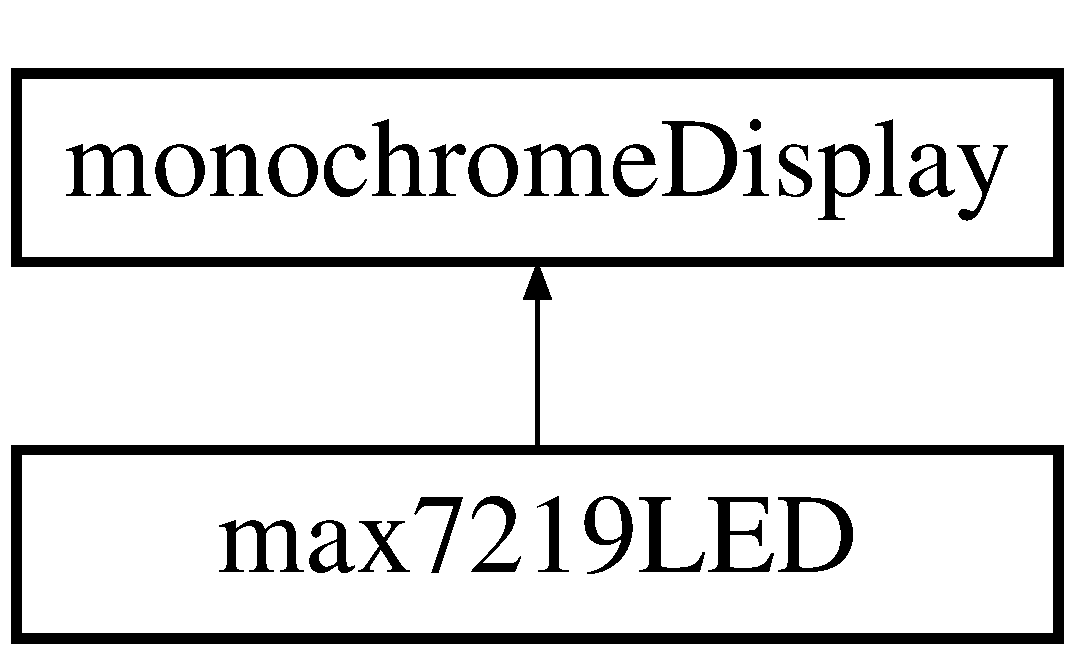
\includegraphics[height=2.000000cm]{classmonochrome_display}
\end{center}
\end{figure}
\subsection*{Public Member Functions}
\begin{DoxyCompactItemize}
\item 
{\bfseries monochrome\+Display} (const int \&size\+\_\+x, const int \&size\+\_\+y)\hypertarget{classmonochrome_display_afdfb66cfcaca269751ff2db466335055}{}\label{classmonochrome_display_afdfb66cfcaca269751ff2db466335055}

\item 
virtual void {\bfseries draw\+Pixel} (int x, int y, int matrix\mbox{[}\hyperlink{max7219_l_e_dconstants_8hpp_a2a4cf20d00f170bb1778318f645ab6cb}{L\+E\+D\+M\+A\+T\+R\+I\+X\+\_\+\+S\+I\+ZE}+1\mbox{]}\mbox{[}(\hyperlink{max7219_l_e_dconstants_8hpp_a2a4cf20d00f170bb1778318f645ab6cb}{L\+E\+D\+M\+A\+T\+R\+I\+X\+\_\+\+S\+I\+ZE} $\ast$\hyperlink{max7219_l_e_dconstants_8hpp_aa3f1c3f51823e34beb0682e7f799793b}{L\+E\+D\+M\+A\+T\+R\+I\+X\+\_\+\+A\+M\+O\+U\+NT})+1\mbox{]}, int data=1)=0\hypertarget{classmonochrome_display_ae0d92a60755a2924799e04382f41f1f0}{}\label{classmonochrome_display_ae0d92a60755a2924799e04382f41f1f0}

\item 
virtual void {\bfseries clear} (int matrix\mbox{[}\hyperlink{max7219_l_e_dconstants_8hpp_a2a4cf20d00f170bb1778318f645ab6cb}{L\+E\+D\+M\+A\+T\+R\+I\+X\+\_\+\+S\+I\+ZE}+1\mbox{]}\mbox{[}(\hyperlink{max7219_l_e_dconstants_8hpp_a2a4cf20d00f170bb1778318f645ab6cb}{L\+E\+D\+M\+A\+T\+R\+I\+X\+\_\+\+S\+I\+ZE} $\ast$\hyperlink{max7219_l_e_dconstants_8hpp_aa3f1c3f51823e34beb0682e7f799793b}{L\+E\+D\+M\+A\+T\+R\+I\+X\+\_\+\+A\+M\+O\+U\+NT})+1\mbox{]})=0\hypertarget{classmonochrome_display_a4cc51ac0de3ff1dc880df4308b9ab056}{}\label{classmonochrome_display_a4cc51ac0de3ff1dc880df4308b9ab056}

\end{DoxyCompactItemize}
\subsection*{Protected Attributes}
\begin{DoxyCompactItemize}
\item 
const int {\bfseries size\+\_\+x}\hypertarget{classmonochrome_display_a76aee278fd30daf328f081020af3d843}{}\label{classmonochrome_display_a76aee278fd30daf328f081020af3d843}

\item 
const int {\bfseries size\+\_\+y}\hypertarget{classmonochrome_display_ab3eccf828513020fd3e62e23c531d594}{}\label{classmonochrome_display_ab3eccf828513020fd3e62e23c531d594}

\end{DoxyCompactItemize}


\subsection{Detailed Description}
\hyperlink{classmonochrome_display}{monochrome\+Display} class 

This class is abstract. It can be used for inheritance purposes with monochrome displays, such as L\+ED matrices and (old) O\+L\+ED screens. 

The documentation for this class was generated from the following file\+:\begin{DoxyCompactItemize}
\item 
\hyperlink{monochrome_8hpp}{monochrome.\+hpp}\end{DoxyCompactItemize}

\chapter{File Documentation}
\hypertarget{max7219_l_e_d_8cpp}{}\section{max7219\+L\+E\+D.\+cpp File Reference}
\label{max7219_l_e_d_8cpp}\index{max7219\+L\+E\+D.\+cpp@{max7219\+L\+E\+D.\+cpp}}
{\ttfamily \#include \char`\"{}max7219\+L\+E\+D.\+hpp\char`\"{}}\\*
{\ttfamily \#include \char`\"{}max7219\+L\+E\+Dconstants.\+hpp\char`\"{}}\\*
{\ttfamily \#include $<$stdint.\+h$>$}\\*
\subsection*{Functions}
\begin{DoxyCompactItemize}
\item 
void \hyperlink{max7219_l_e_d_8cpp_a1a3100a4e708acfadc2c26d04e7531b9}{pulse\+\_\+clk} (hwlib\+::pin\+\_\+out \&clk)
\begin{DoxyCompactList}\small\item\em Pulse clock. \end{DoxyCompactList}\end{DoxyCompactItemize}


\subsection{Detailed Description}
\hyperlink{classmax7219_l_e_d}{max7219\+L\+ED} constructor 

\subsection{Function Documentation}
\index{max7219\+L\+E\+D.\+cpp@{max7219\+L\+E\+D.\+cpp}!pulse\+\_\+clk@{pulse\+\_\+clk}}
\index{pulse\+\_\+clk@{pulse\+\_\+clk}!max7219\+L\+E\+D.\+cpp@{max7219\+L\+E\+D.\+cpp}}
\subsubsection[{\texorpdfstring{pulse\+\_\+clk(hwlib\+::pin\+\_\+out \&clk)}{pulse_clk(hwlib::pin_out &clk)}}]{\setlength{\rightskip}{0pt plus 5cm}void pulse\+\_\+clk (
\begin{DoxyParamCaption}
\item[{hwlib\+::pin\+\_\+out \&}]{clk}
\end{DoxyParamCaption}
)}\hypertarget{max7219_l_e_d_8cpp_a1a3100a4e708acfadc2c26d04e7531b9}{}\label{max7219_l_e_d_8cpp_a1a3100a4e708acfadc2c26d04e7531b9}


Pulse clock. 

This function pulses the clock 
\hypertarget{max7219_l_e_d_8hpp}{}\section{max7219\+L\+E\+D.\+hpp File Reference}
\label{max7219_l_e_d_8hpp}\index{max7219\+L\+E\+D.\+hpp@{max7219\+L\+E\+D.\+hpp}}
{\ttfamily \#include \char`\"{}monochrome.\+hpp\char`\"{}}\\*
{\ttfamily \#include \char`\"{}hwlib.\+hpp\char`\"{}}\\*
{\ttfamily \#include \char`\"{}max7219\+L\+E\+Dconstants.\+hpp\char`\"{}}\\*
\subsection*{Classes}
\begin{DoxyCompactItemize}
\item 
class \hyperlink{classmax7219_l_e_d}{max7219\+L\+ED}
\begin{DoxyCompactList}\small\item\em \hyperlink{classmax7219_l_e_d}{max7219\+L\+ED} class \end{DoxyCompactList}\end{DoxyCompactItemize}
\subsection*{Functions}
\begin{DoxyCompactItemize}
\item 
void \hyperlink{max7219_l_e_d_8hpp_a1a3100a4e708acfadc2c26d04e7531b9}{pulse\+\_\+clk} (hwlib\+::pin\+\_\+out \&clk)
\begin{DoxyCompactList}\small\item\em Pulse clock. \end{DoxyCompactList}\end{DoxyCompactItemize}


\subsection{Function Documentation}
\index{max7219\+L\+E\+D.\+hpp@{max7219\+L\+E\+D.\+hpp}!pulse\+\_\+clk@{pulse\+\_\+clk}}
\index{pulse\+\_\+clk@{pulse\+\_\+clk}!max7219\+L\+E\+D.\+hpp@{max7219\+L\+E\+D.\+hpp}}
\subsubsection[{\texorpdfstring{pulse\+\_\+clk(hwlib\+::pin\+\_\+out \&clk)}{pulse_clk(hwlib::pin_out &clk)}}]{\setlength{\rightskip}{0pt plus 5cm}void pulse\+\_\+clk (
\begin{DoxyParamCaption}
\item[{hwlib\+::pin\+\_\+out \&}]{clk}
\end{DoxyParamCaption}
)}\hypertarget{max7219_l_e_d_8hpp_a1a3100a4e708acfadc2c26d04e7531b9}{}\label{max7219_l_e_d_8hpp_a1a3100a4e708acfadc2c26d04e7531b9}


Pulse clock. 

This function pulses the clock. 
\hypertarget{max7219_l_e_dconstants_8hpp}{}\section{max7219\+L\+E\+Dconstants.\+hpp File Reference}
\label{max7219_l_e_dconstants_8hpp}\index{max7219\+L\+E\+Dconstants.\+hpp@{max7219\+L\+E\+Dconstants.\+hpp}}
\subsection*{Variables}
\begin{DoxyCompactItemize}
\item 
constexpr uint8\+\_\+t \hyperlink{max7219_l_e_dconstants_8hpp_a408fbf1a6ed4eb62332d21409dde461e}{M\+A\+X7219\+\_\+\+R\+E\+G\+\_\+\+N\+O\+\_\+\+OP} = 0x00\hypertarget{max7219_l_e_dconstants_8hpp_a408fbf1a6ed4eb62332d21409dde461e}{}\label{max7219_l_e_dconstants_8hpp_a408fbf1a6ed4eb62332d21409dde461e}

\begin{DoxyCompactList}\small\item\em N\+O-\/\+OP register address -\/ If this is send as an address, the matrix this is sent to changes nothing, disregarding the data sent to the same chip. \end{DoxyCompactList}\item 
constexpr uint8\+\_\+t \hyperlink{max7219_l_e_dconstants_8hpp_af20cb867bf5eee163e0f7661377870c7}{M\+A\+X7219\+\_\+\+R\+E\+G\+\_\+\+D\+E\+C\+O\+DE} = 0x09\hypertarget{max7219_l_e_dconstants_8hpp_af20cb867bf5eee163e0f7661377870c7}{}\label{max7219_l_e_dconstants_8hpp_af20cb867bf5eee163e0f7661377870c7}

\begin{DoxyCompactList}\small\item\em D\+E\+C\+O\+DE register address -\/ Sets the decode mode of the max7219 chip. \end{DoxyCompactList}\item 
constexpr uint8\+\_\+t {\bfseries M\+A\+X7219\+\_\+\+R\+E\+G\+\_\+\+B\+R\+I\+G\+H\+T\+N\+E\+SS} = 0x0A\hypertarget{max7219_l_e_dconstants_8hpp_aecd4be0e26c3c0e1b5cd6fc87a1a51d2}{}\label{max7219_l_e_dconstants_8hpp_aecd4be0e26c3c0e1b5cd6fc87a1a51d2}

\item 
constexpr uint8\+\_\+t {\bfseries M\+A\+X7219\+\_\+\+R\+E\+G\+\_\+\+S\+C\+A\+N\+\_\+\+L\+I\+M\+IT} = 0x0B\hypertarget{max7219_l_e_dconstants_8hpp_a661e5f37d9ba732e7f00d307a60634d5}{}\label{max7219_l_e_dconstants_8hpp_a661e5f37d9ba732e7f00d307a60634d5}

\item 
constexpr uint8\+\_\+t {\bfseries M\+A\+X7219\+\_\+\+R\+E\+G\+\_\+\+S\+H\+U\+T\+D\+O\+WN} = 0x0C\hypertarget{max7219_l_e_dconstants_8hpp_a17b37a9a9308cd302fec821582a5c175}{}\label{max7219_l_e_dconstants_8hpp_a17b37a9a9308cd302fec821582a5c175}

\item 
constexpr uint8\+\_\+t {\bfseries M\+A\+X7219\+\_\+\+R\+E\+G\+\_\+\+D\+I\+S\+P\+L\+A\+Y\+T\+E\+ST} = 0x0F\hypertarget{max7219_l_e_dconstants_8hpp_aca2bbd40158450011549c88bc53dc4a5}{}\label{max7219_l_e_dconstants_8hpp_aca2bbd40158450011549c88bc53dc4a5}

\item 
constexpr uint8\+\_\+t {\bfseries M\+A\+X7219\+\_\+\+C\+O\+L\+U\+M\+N1} = 0x01\hypertarget{max7219_l_e_dconstants_8hpp_a2dac53900bd71b295133bf989053490c}{}\label{max7219_l_e_dconstants_8hpp_a2dac53900bd71b295133bf989053490c}

\item 
constexpr uint8\+\_\+t {\bfseries M\+A\+X7219\+\_\+\+C\+O\+L\+U\+M\+N2} = 0x02\hypertarget{max7219_l_e_dconstants_8hpp_a3358cf3fecdb1d0a84b8c90e095e9c08}{}\label{max7219_l_e_dconstants_8hpp_a3358cf3fecdb1d0a84b8c90e095e9c08}

\item 
constexpr uint8\+\_\+t {\bfseries M\+A\+X7219\+\_\+\+C\+O\+L\+U\+M\+N3} = 0x03\hypertarget{max7219_l_e_dconstants_8hpp_a01830d85b977b122d711baeda96e9969}{}\label{max7219_l_e_dconstants_8hpp_a01830d85b977b122d711baeda96e9969}

\item 
constexpr uint8\+\_\+t {\bfseries M\+A\+X7219\+\_\+\+C\+O\+L\+U\+M\+N4} = 0x04\hypertarget{max7219_l_e_dconstants_8hpp_aa4c36b2978acff501a88284305bf2f93}{}\label{max7219_l_e_dconstants_8hpp_aa4c36b2978acff501a88284305bf2f93}

\item 
constexpr uint8\+\_\+t {\bfseries M\+A\+X7219\+\_\+\+C\+O\+L\+U\+M\+N5} = 0x05\hypertarget{max7219_l_e_dconstants_8hpp_a3f5ab51577c409f3e34dcca8631bef2c}{}\label{max7219_l_e_dconstants_8hpp_a3f5ab51577c409f3e34dcca8631bef2c}

\item 
constexpr uint8\+\_\+t {\bfseries M\+A\+X7219\+\_\+\+C\+O\+L\+U\+M\+N6} = 0x06\hypertarget{max7219_l_e_dconstants_8hpp_aa519c1ed3a3c022c6786dfd6771d2582}{}\label{max7219_l_e_dconstants_8hpp_aa519c1ed3a3c022c6786dfd6771d2582}

\item 
constexpr uint8\+\_\+t {\bfseries M\+A\+X7219\+\_\+\+C\+O\+L\+U\+M\+N7} = 0x07\hypertarget{max7219_l_e_dconstants_8hpp_a81470f8772ed288a262120e9d3bdbc28}{}\label{max7219_l_e_dconstants_8hpp_a81470f8772ed288a262120e9d3bdbc28}

\item 
constexpr uint8\+\_\+t {\bfseries M\+A\+X7219\+\_\+\+C\+O\+L\+U\+M\+N8} = 0x08\hypertarget{max7219_l_e_dconstants_8hpp_a19625a4163531ef9bb20137e017a54cf}{}\label{max7219_l_e_dconstants_8hpp_a19625a4163531ef9bb20137e017a54cf}

\item 
constexpr uint8\+\_\+t \hyperlink{max7219_l_e_dconstants_8hpp_a880074d5cf17d63d929589243cf6733b}{M\+A\+X7219\+\_\+\+N\+O\+\_\+\+O\+P\+\_\+\+D\+A\+TA} = 0x00\hypertarget{max7219_l_e_dconstants_8hpp_a880074d5cf17d63d929589243cf6733b}{}\label{max7219_l_e_dconstants_8hpp_a880074d5cf17d63d929589243cf6733b}

\begin{DoxyCompactList}\small\item\em Multi-\/purpose data -\/ Sends no data to a column or used for a N\+O-\/\+OP on certain settings. \end{DoxyCompactList}\item 
constexpr uint8\+\_\+t \hyperlink{max7219_l_e_dconstants_8hpp_a11b0693c95789d864ef1a57ff92d4353}{M\+A\+X7219\+\_\+\+S\+C\+A\+N\+\_\+\+L\+I\+M\+IT} = 0x07\hypertarget{max7219_l_e_dconstants_8hpp_a11b0693c95789d864ef1a57ff92d4353}{}\label{max7219_l_e_dconstants_8hpp_a11b0693c95789d864ef1a57ff92d4353}

\begin{DoxyCompactList}\small\item\em Sets the amount of columns that can be adressed, 1-\/8 (0x00-\/0x07). \end{DoxyCompactList}\item 
constexpr uint8\+\_\+t \hyperlink{max7219_l_e_dconstants_8hpp_a41139ac4b2879f2f560ff2e47087303b}{M\+A\+X7219\+\_\+\+N\+O\+R\+M\+A\+L\+\_\+\+O\+P\+E\+R\+A\+T\+I\+ON} = 0x01\hypertarget{max7219_l_e_dconstants_8hpp_a41139ac4b2879f2f560ff2e47087303b}{}\label{max7219_l_e_dconstants_8hpp_a41139ac4b2879f2f560ff2e47087303b}

\begin{DoxyCompactList}\small\item\em Used to enable Shutdown mode and Display test. \end{DoxyCompactList}\item 
constexpr uint8\+\_\+t \hyperlink{max7219_l_e_dconstants_8hpp_af94bcc4ac3a0265d7d8264d575cfa763}{B\+R\+I\+G\+H\+T\+N\+E\+S\+S\+\_\+\+L\+VL} = 0x01\hypertarget{max7219_l_e_dconstants_8hpp_af94bcc4ac3a0265d7d8264d575cfa763}{}\label{max7219_l_e_dconstants_8hpp_af94bcc4ac3a0265d7d8264d575cfa763}

\begin{DoxyCompactList}\small\item\em Sets brightness of L\+E\+Ds (0x01-\/0x1F). \end{DoxyCompactList}\item 
constexpr uint8\+\_\+t \hyperlink{max7219_l_e_dconstants_8hpp_aa3f1c3f51823e34beb0682e7f799793b}{L\+E\+D\+M\+A\+T\+R\+I\+X\+\_\+\+A\+M\+O\+U\+NT} = 4\hypertarget{max7219_l_e_dconstants_8hpp_aa3f1c3f51823e34beb0682e7f799793b}{}\label{max7219_l_e_dconstants_8hpp_aa3f1c3f51823e34beb0682e7f799793b}

\begin{DoxyCompactList}\small\item\em Sets the amount of L\+ED matrices daisy chained. \end{DoxyCompactList}\item 
constexpr uint8\+\_\+t \hyperlink{max7219_l_e_dconstants_8hpp_a2a4cf20d00f170bb1778318f645ab6cb}{L\+E\+D\+M\+A\+T\+R\+I\+X\+\_\+\+S\+I\+ZE} = 8\hypertarget{max7219_l_e_dconstants_8hpp_a2a4cf20d00f170bb1778318f645ab6cb}{}\label{max7219_l_e_dconstants_8hpp_a2a4cf20d00f170bb1778318f645ab6cb}

\begin{DoxyCompactList}\small\item\em Sets the size of the led matrices. \end{DoxyCompactList}\item 
constexpr uint8\+\_\+t {\bfseries P\+I\+X\+E\+L\+B\+U\+F\+F\+ER} = 0x00\hypertarget{max7219_l_e_dconstants_8hpp_adaf41fa8ea78b78c230b891420580d0d}{}\label{max7219_l_e_dconstants_8hpp_adaf41fa8ea78b78c230b891420580d0d}

\end{DoxyCompactItemize}

\hypertarget{monochrome_8hpp}{}\section{monochrome.\+hpp File Reference}
\label{monochrome_8hpp}\index{monochrome.\+hpp@{monochrome.\+hpp}}
{\ttfamily \#include $<$stdint.\+h$>$}\\*
{\ttfamily \#include \char`\"{}max7219\+L\+E\+Dconstants.\+hpp\char`\"{}}\\*
\subsection*{Classes}
\begin{DoxyCompactItemize}
\item 
class \hyperlink{classmonochrome_display}{monochrome\+Display}
\begin{DoxyCompactList}\small\item\em \hyperlink{classmonochrome_display}{monochrome\+Display} class \end{DoxyCompactList}\end{DoxyCompactItemize}

%--- End generated contents ---

% Index
\backmatter
\newpage
\phantomsection
\clearemptydoublepage
\addcontentsline{toc}{chapter}{Index}
\printindex

\end{document}
